
Se toma como referencia la~\cref{fig:hexagonalDiagram}, el diagrama más extendido de ejemplo para una arquitectura hexagonal, para una explicación de alto nivel para la funcionalidad de crear tareas \textit{CreateTaskUseCase} que se aprecia en la~\cref{fig:CreateTaskHexagonalDiagram}.
Los componentes que intervienen son:
\begin{itemize}
    \item \textit{WebAdapter}: contiene la lógica relacionada con la recepción de llamadas RPC está ligada a la infraestructura necesaria para ello, es decir importa las librerías para ello.
    A través de una interfaz se le ha de inyectar un puerto de entrada que le permita ejecutar la lógica del caso de uso.
    \item UseCase: contiene la lógica necesaria para garantizar la correcta llamada a la lógica de Dominio para la creación de una Tarea.
    Contiene las verificaciones, mediante la instanciación, entre los tipos primitivos y los objetos de Dominio.
    \item \textit{Creator}: servicio de creación de tareas.
    Contiene la lógica que obligatoriamente ha de ejecutarse de forma simultanea cuando se crea una tarea.
    La persistencia en la base de datos a través de un puerto de salida; una interfaz que se le inyecta y le permite ejecutar dicha lógica sin conocerla.
    También de emite un evento de Dominio comunicando la creación mediante el acceso a un puerto de salida.
    \item \textit{PersistenceAdapter}: contiene la lógica relacionada con la persistencia de datos.
    está ligado a la infraestructura de la base de datos y contiene por tanto las importaciones de las librerías necesarias.
    \item \textit{DispatcherAdapter}: este puerto de salida contiene la lógica para gestionar los eventos emitidos por el dominio.
    Para ello, necesita que le sean inyectados los casos de uso, eventHandler en este caso al no ser ejecutados directamente por un usuario.
    De esta forma, a la vez que un puerto de salida se convierte en un Adaptador de entrada que ejecuta puertos de entrada de nuevo a la aplicación.
    \item \textit{Looper}: Contiene la lógica necesaria para obtener de base de datos, a través de un puerto de salida, todas las tareas sobre las que hay que iterar para ejecutarlas.
    \item \textit{Entity}: en este caso de uso serán las Tareas (\textit{Tasks})
\end{itemize}

Encontramos en la figura la numeración en orden de ejecución.
\begin{enumerate}
    \item se recibe una llamada RPC de tipo \textit{CreateTask} mediante el WebAdapter y es atendida
    \item A través de puerto de entrada se ejecuta el caso de uso
    \item El caso de uso instancia los elementos de Dominio necesarios y ejecuta el servicio \textit{Creator}
    \item El servicio \textit{Creator} comunica la información a persistir a través del puerto de salida
    \item La interfaz del el Adaptador de persistencia que ha de ser inyectada en el \textit{Creator}
    \item El componente inyectado en el \textit{Creator} que cumple con la interfaz 5 persiste la información en base de datos
    \item El servicio \textit{Creator} comunica el evento de creación a través del puerto de salida 7
    \item El servicio \textit{Dispatcher} inyectado en el creator que cumple con la interfaz 7 ejecuta el caso de uso correspondiente a ese evento a través de la interfaz
    \item La interfaz del caso de uso, en este caso \textit{eventHandler} de la creación de tareas
    \item El caso de uso que gestiona los eventos de creación de tareas.
    Cumple con la interfaz 9 y se encarga de comprobar que si el tipo de tarea creada requiere la activación del servicio de ejecución.
    \item El servicio de ejecución de tareas automáticas o \textit{Looper}.
    Se encarga de obtener a través de el puerto de salida 5, de la base de datos, y ejecutar todas las tareas definidas como automáticas.
\end{enumerate}

\begin{figure}[H]
    \centering
    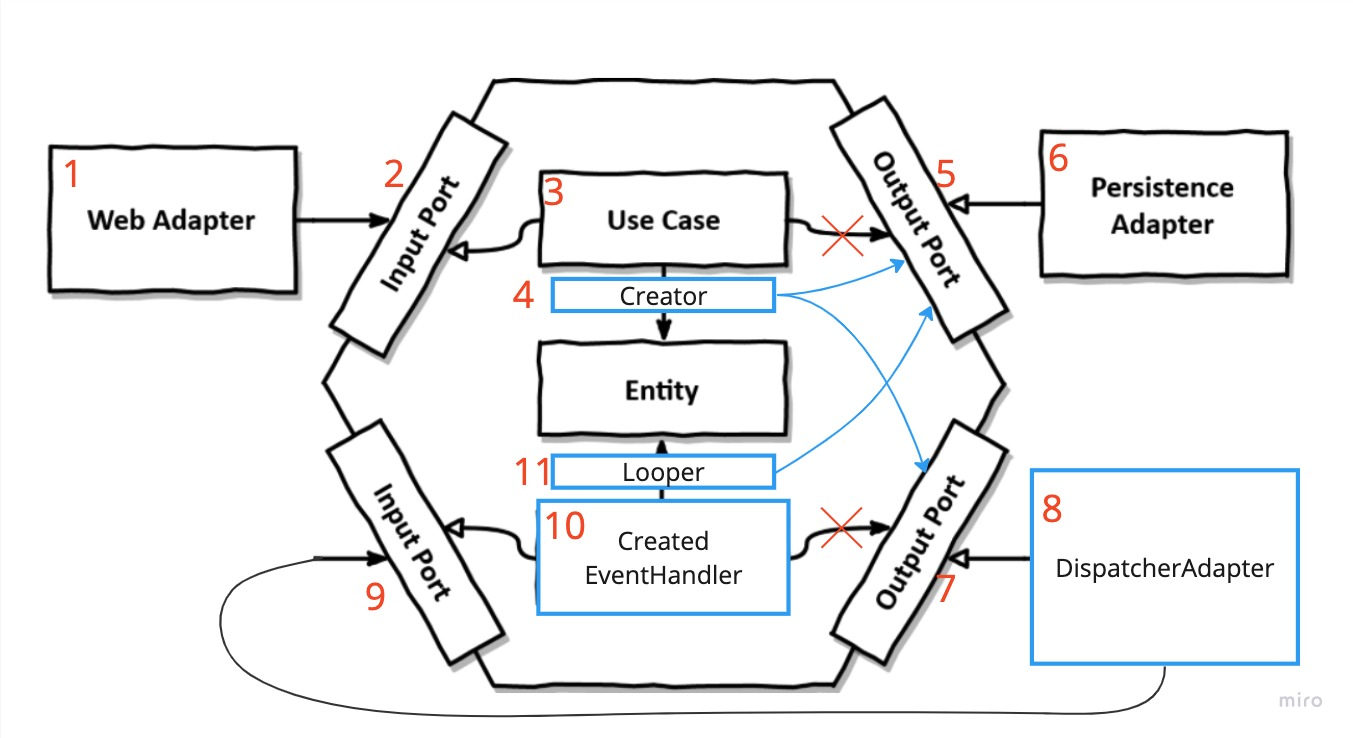
\includegraphics[height=0.3\textheight]{./part/Ejecucion/Seguimiento/CreateTaskUseCase/img/CreateTaskHexagonalDiagram}
    \caption{Hexagonal architecture diagram}\label{fig:CreateTaskHexagonalDiagram}
\end{figure}

Se puede apreciar que el UL ayuda a la comprensión de los pasos y las funcionalidades.
El diseño ayuda a diferenciar la resolución del problema: representado por la creación de tareas y su ejecución.
Separando el porqué y dónde se ejecuta: se activa la resolución del problema por una llamada RPC, en una Base de datos y en un sistema remoto.
Si cualquiera de los elementos que acceden a el programa que resuelve el caso de uso quiere ser intercambiado, la única exigencia es implementar las interfaces requeridas por la aplicación.

La implementación concreta para componer la aplicación correspondiente a este caso de uso la encontramos en el~\cref{lst:bootstrapingExample}.
El orden de instanciación e inyección de cada uno de los componentes necesarios para el armado de la aplicación se vuelve un poco más confuso a la hora de llevarlo a la práctica, es por esto que los ejemplos gráficos son de gran ayuda.

\phantom{blank}
\vspace{10mm}
\hrule
\begin{lstlisting}[language=Go,caption={Ejemplo de \textit{Bootstraping} del sistema },breaklines=true,label={lst:bootstrapingExample}]

package Bootstrap

func Bootstrap() {
    //infra
    var persistenceAdapter := PersistenceAdapter.New(<infra dependencies>)
    //Domain
    var looper := Looper.New(persistenceAdapter)
    var createdEventHandler := CreatedEventHandler(looper)
    //Application
    var dispatcherAdapter := DispatcherAdapter.New(createdEventHandler)
    //Domain
    var creator := creator.New(dispatcherAdapter)
    //Application
    var useCase := UseCase.New(creator)
    //Infra
    var webAdapter := WebAdapter.New(<infra dependencies>,useCase)
}

\end{lstlisting}
\hrule

Para una explicación conceptual de la arquitectura como técnica de diseño los diagramas hexagonales pueden tener un valor didáctico, sin embargo, para un caso de uso más completo como el que desarrolla esta sección pierde el sentido.
No logra ser explicativo, ya que hay puertos de salida que se convierten en puertos de entrada como es el caso del Dispatcher, y al quitar lógica de negocio del caso de uso mediante servicios de dominio que impidan el acceso directo a los repositorios de persistencia dicho diagrama se va quedando pequeño.
Es preferible diagramas UML completos como el desarrollado en la~\cref{fig:createTaskUseCaseArchitecture}.
En el diagrama~\cref{fig:createTaskUseCaseArchitectureFolderStructure} se muestra interacción de componentes atendiendo a su distribución en nuestro diseño organizativo del código en ficheros.

Como estrategia de mapeo entre capas o \textit{mapping} Go casi obliga al uso general de interfaces entre todos los elementos, incluidos las clases.
Al necesitar el equivalente de la implementación de clase para garantizar la cohesión ya se hace uso de  interfaces para todos los elementos.
En el desarrollo de la aplicación se ha optado por una estrategia \textit{Full Mapping} con adaptaciones.
Dentro de la estrategia \textit{Full Mapping} se debe implementar un modelo tanto de entrada, como ya se contempla, como de salida.
Es decir, la respuesta que hay entre cada capa también debe ser mapeada mediante un DTO, el patrón adaptado se muestra en la figura~\cref{fig:GetHandMapping}

Esto aumenta la burocracia y finalmente la opción implementada ha sido una adaptación personalizada que se muestra en la figura~\cref{fig:CreateTaskUseCaseMapping}.
En rojo se han marcado los atajos que se han tomado, es decir, el mapeo que no se ha implementado.
El objetivo es aislar bien de los puertos de entrada, es decir el GRPC, y no tanto de los puertos de salida;
ya que la persistencia está bien aislada mediante las interfaces y somos propietarios y consumidores internos de ellas.
Al ser los únicos consumidores de los puertos de salida se dispone de más libertad de cambio sin afectar a terceros.
Dentro de los adaptadores se hace el trabajo de mapeo entre las entidades de dominio y los modelos de persistencia; traduciendo de nuevo a dominio para responder.

\begin{figure}[H]
    \centering
    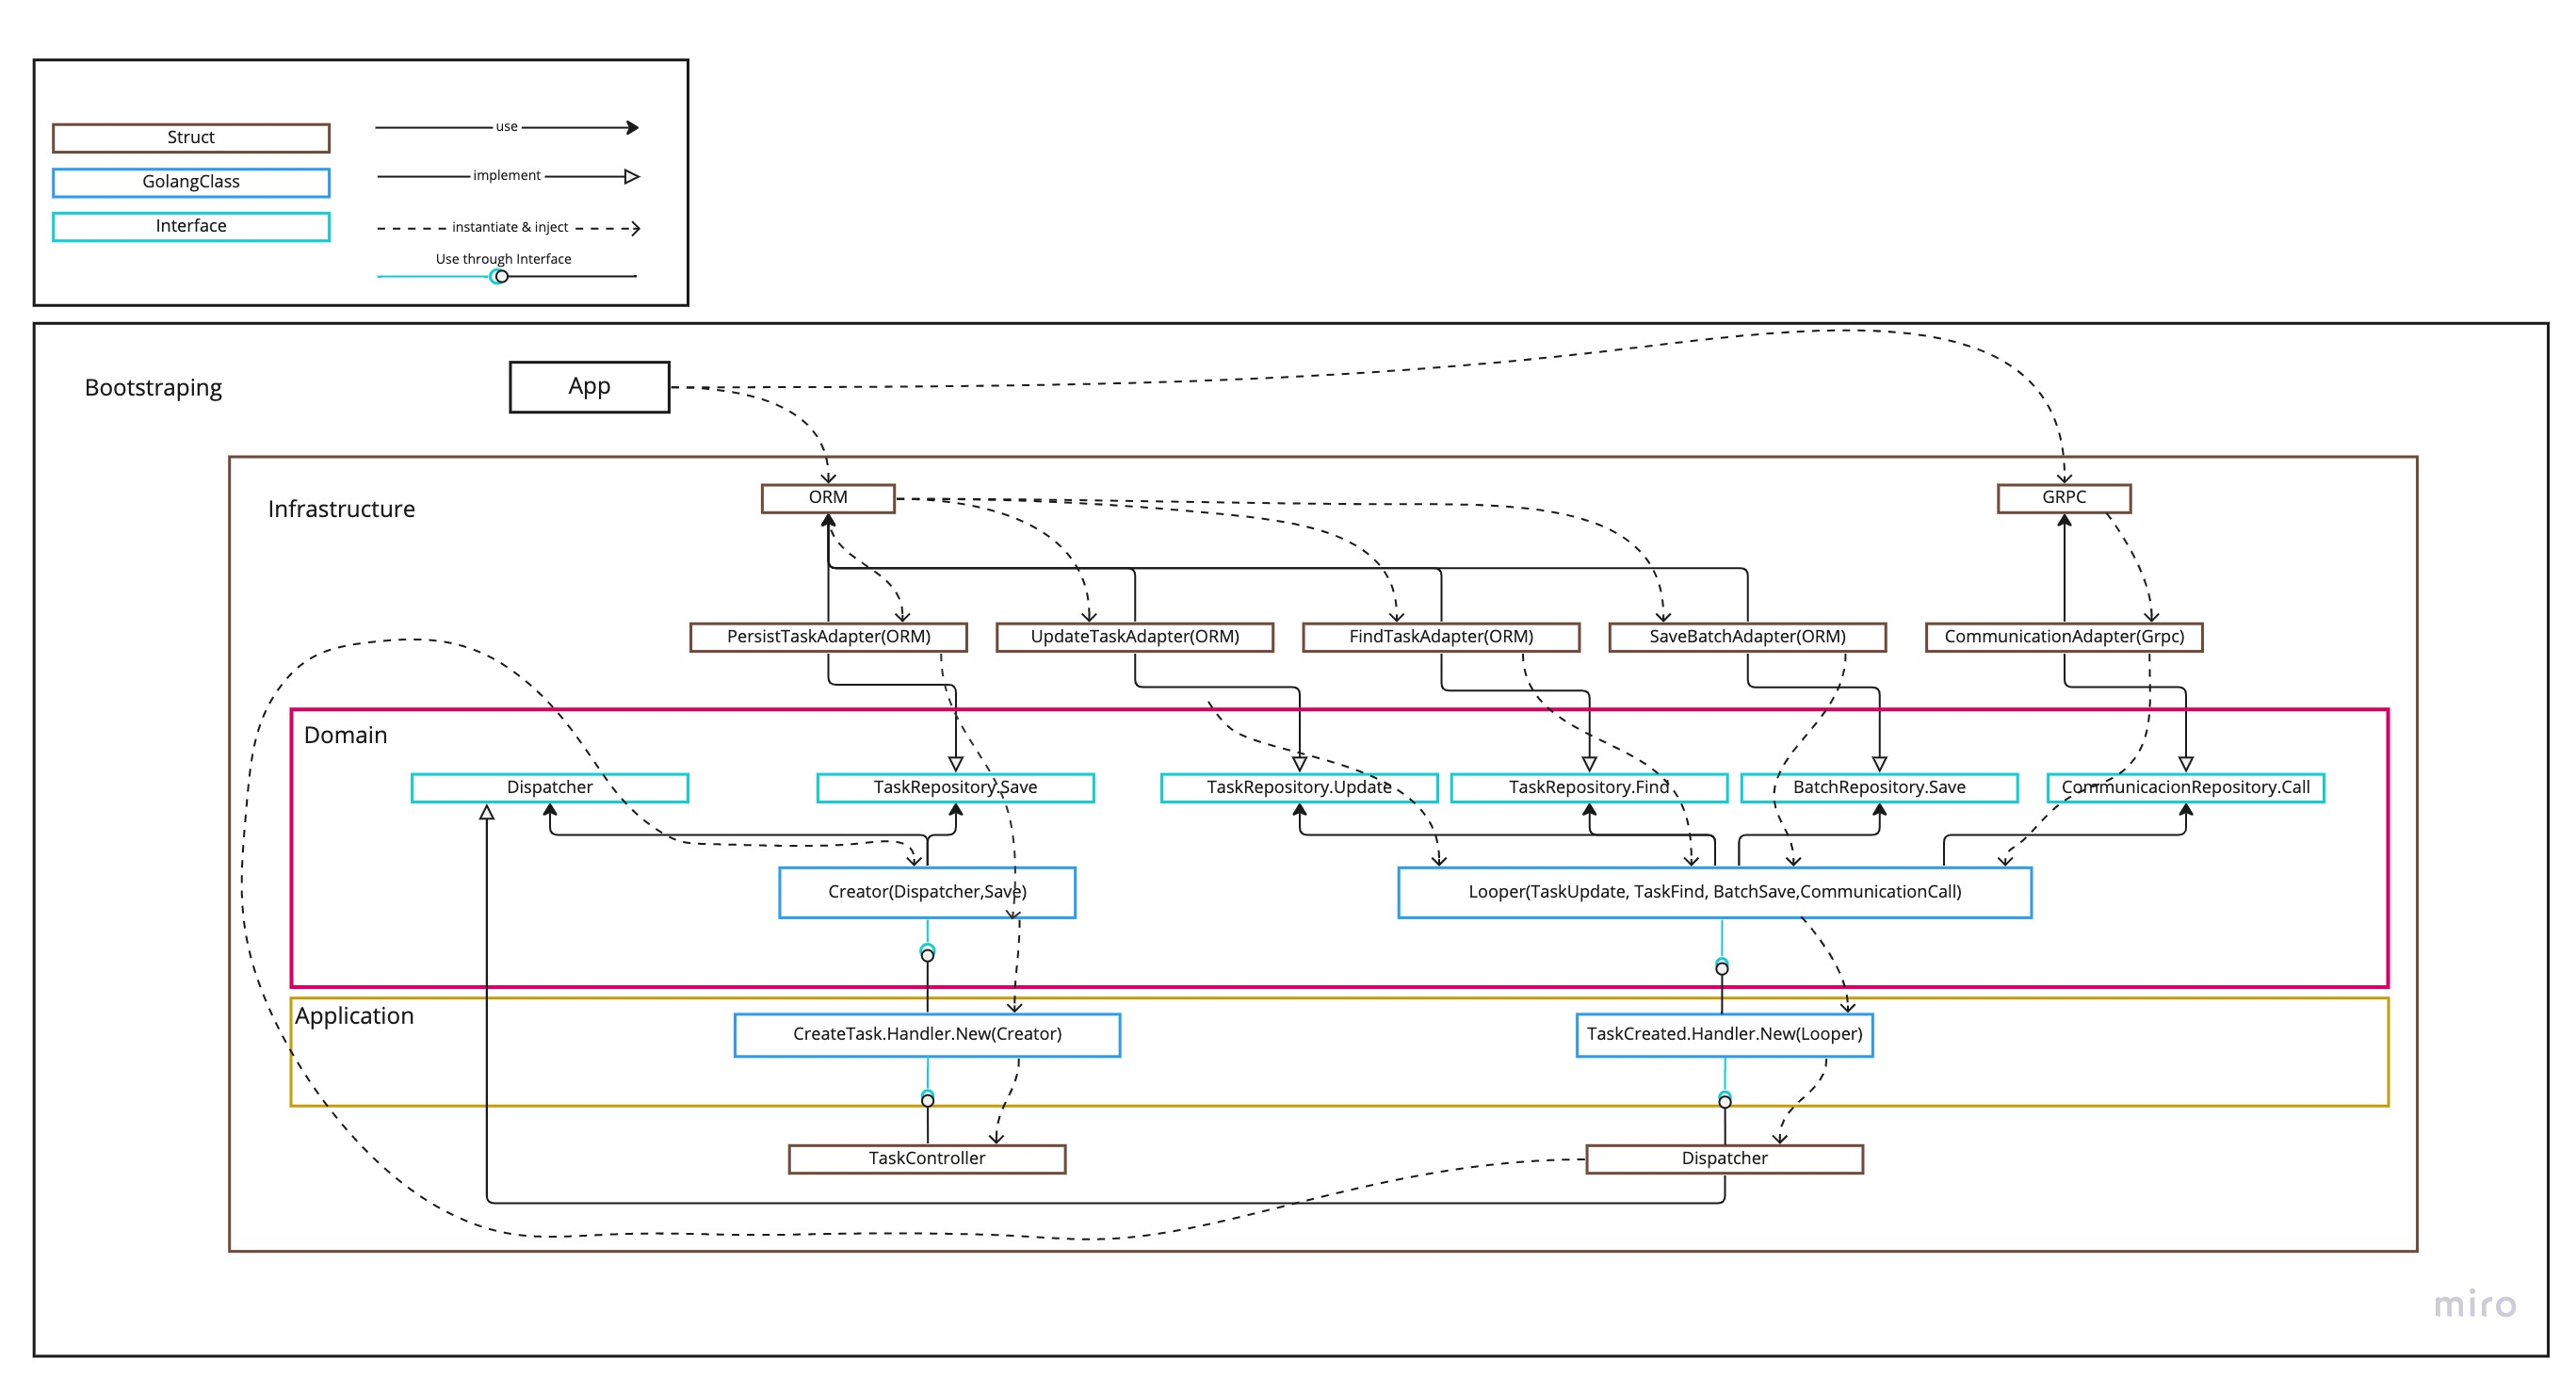
\includegraphics[angle=90,height=1\textheight]{./part/Ejecucion/Seguimiento/CreateTaskUseCase/img/createTaskUseCaseArchitecture}
    \caption{CreateTaskUseCase hexagonal architecture diagram}\label{fig:createTaskUseCaseArchitecture}
\end{figure}

\begin{figure}[H]
    \centering
    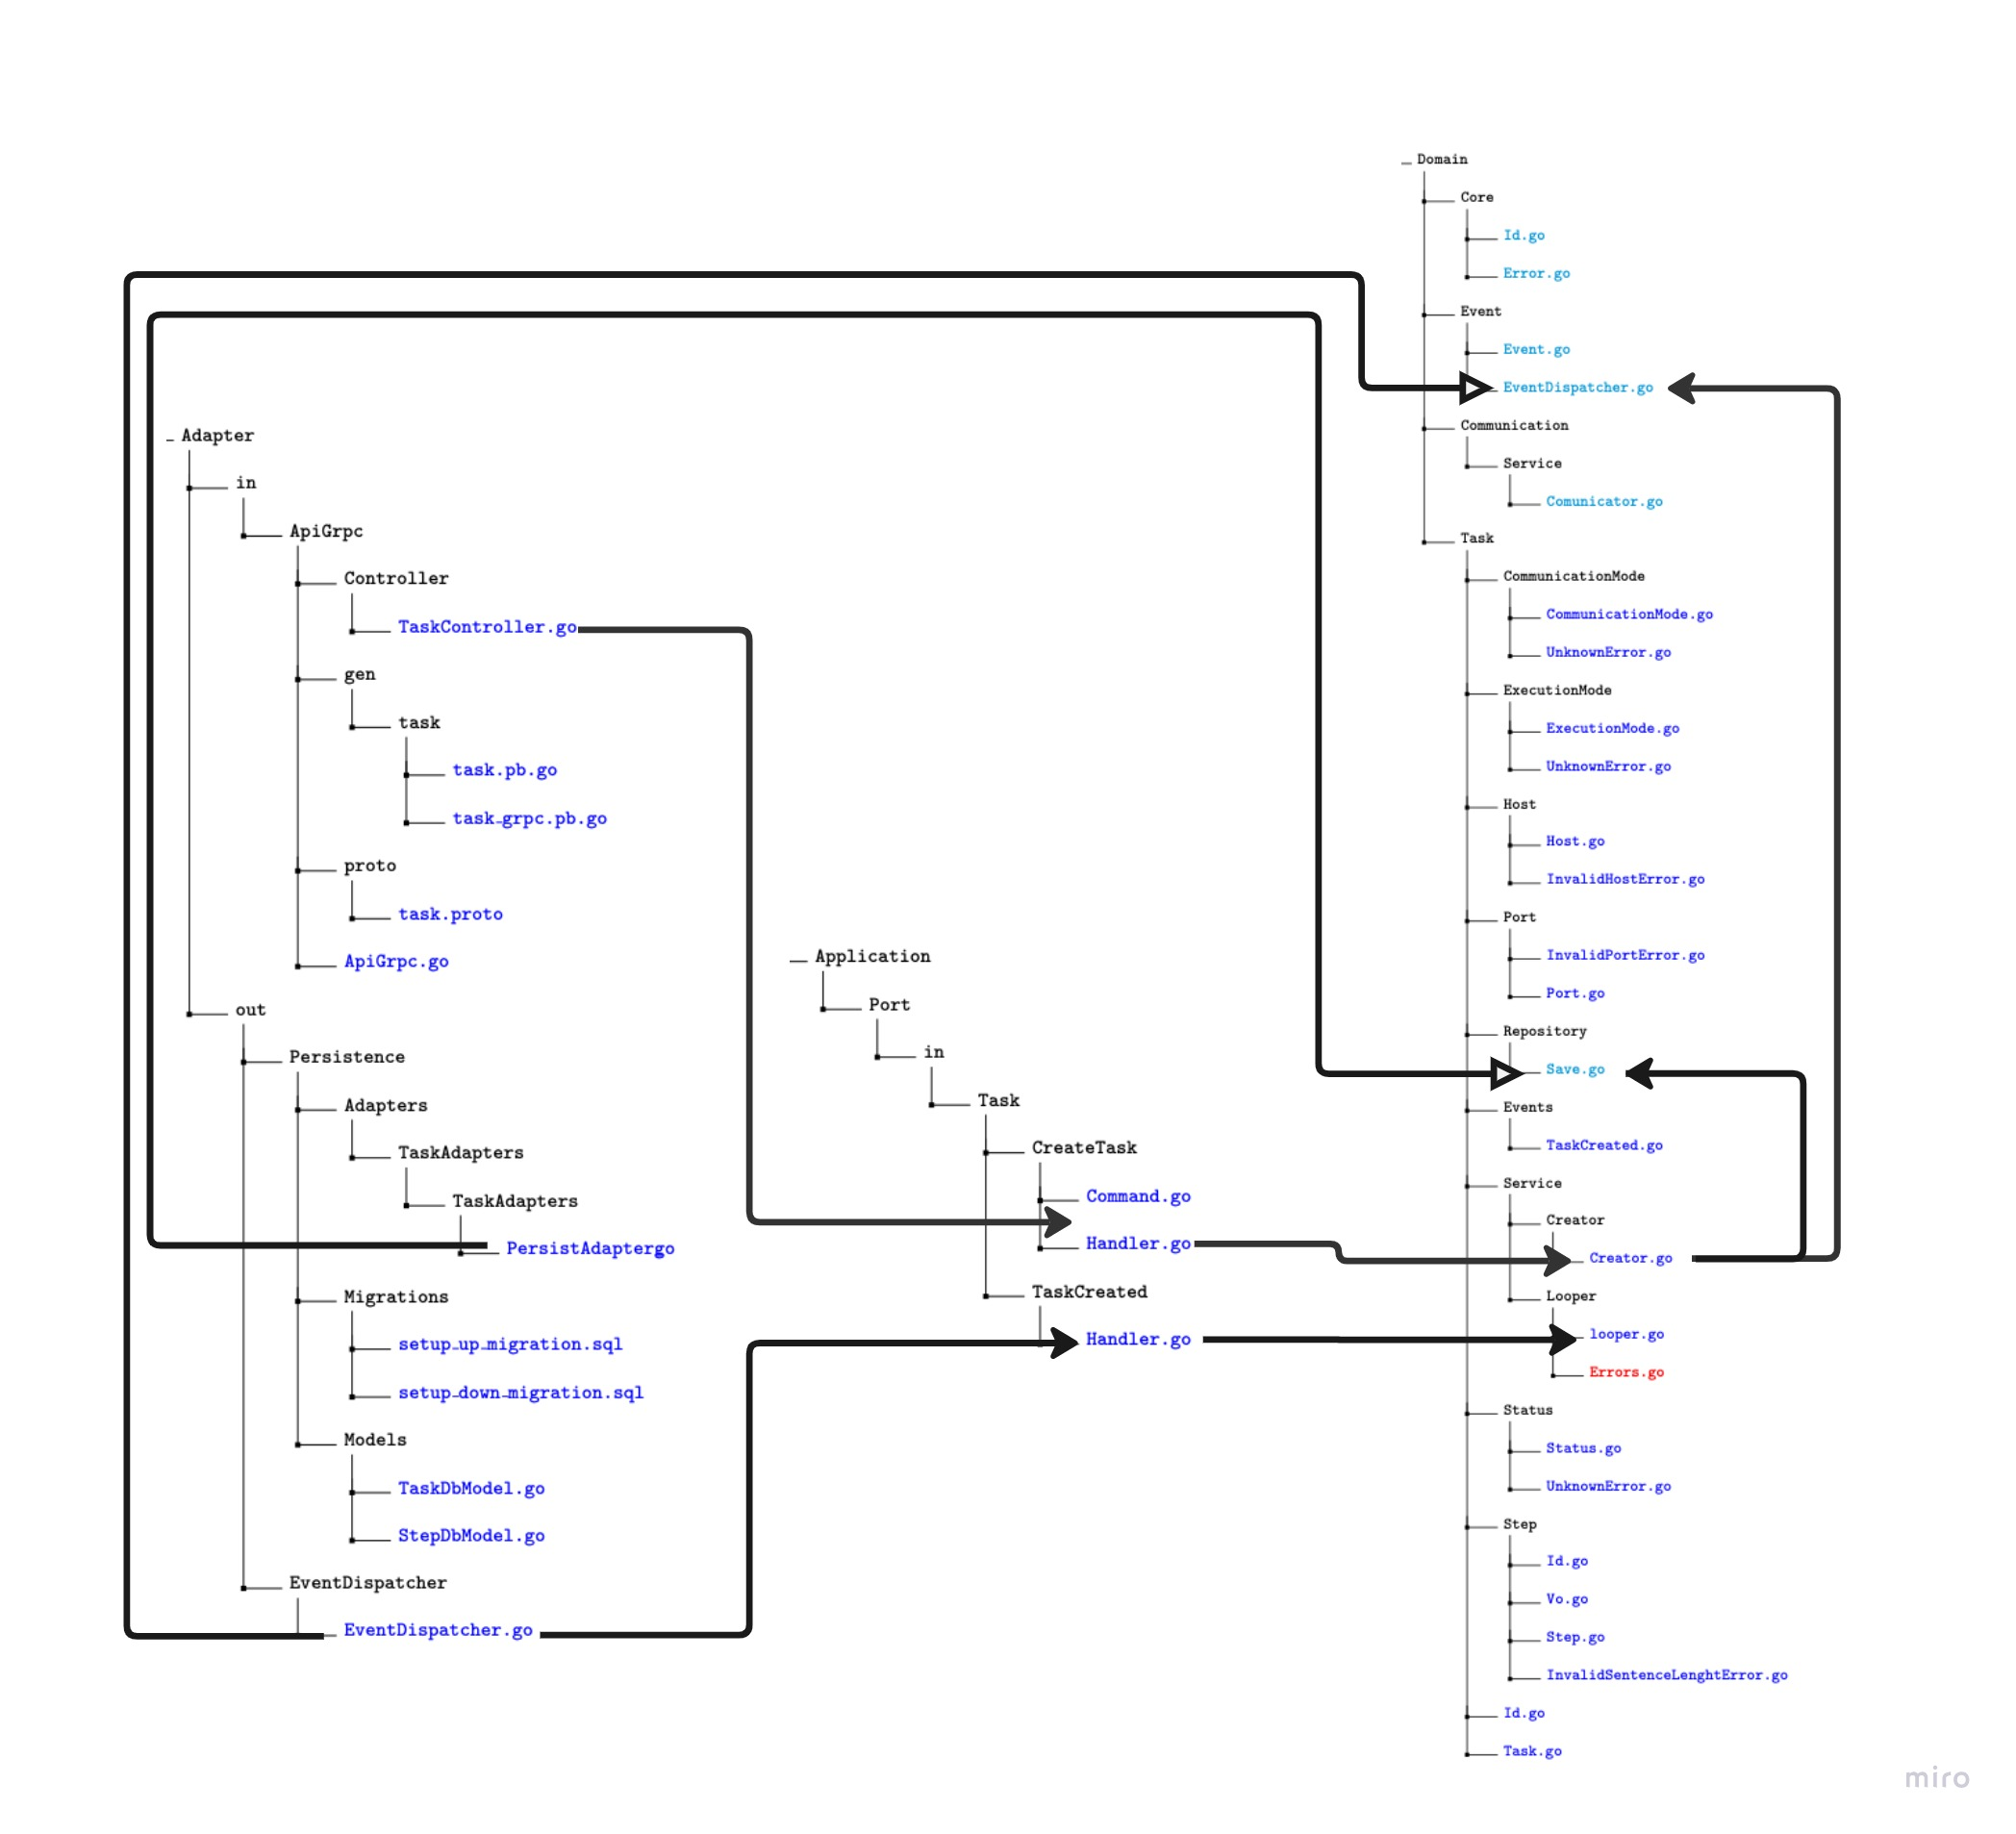
\includegraphics[height=0.5\textheight]{./part/Ejecucion/Seguimiento/CreateTaskUseCase/img/PFM - CreateUseCaseFolderStructure}
    \caption{CreateTaskUseCase folder Structure}\label{fig:createTaskUseCaseArchitectureFolderStructure}
\end{figure}

\begin{figure}[H]
    \centering
    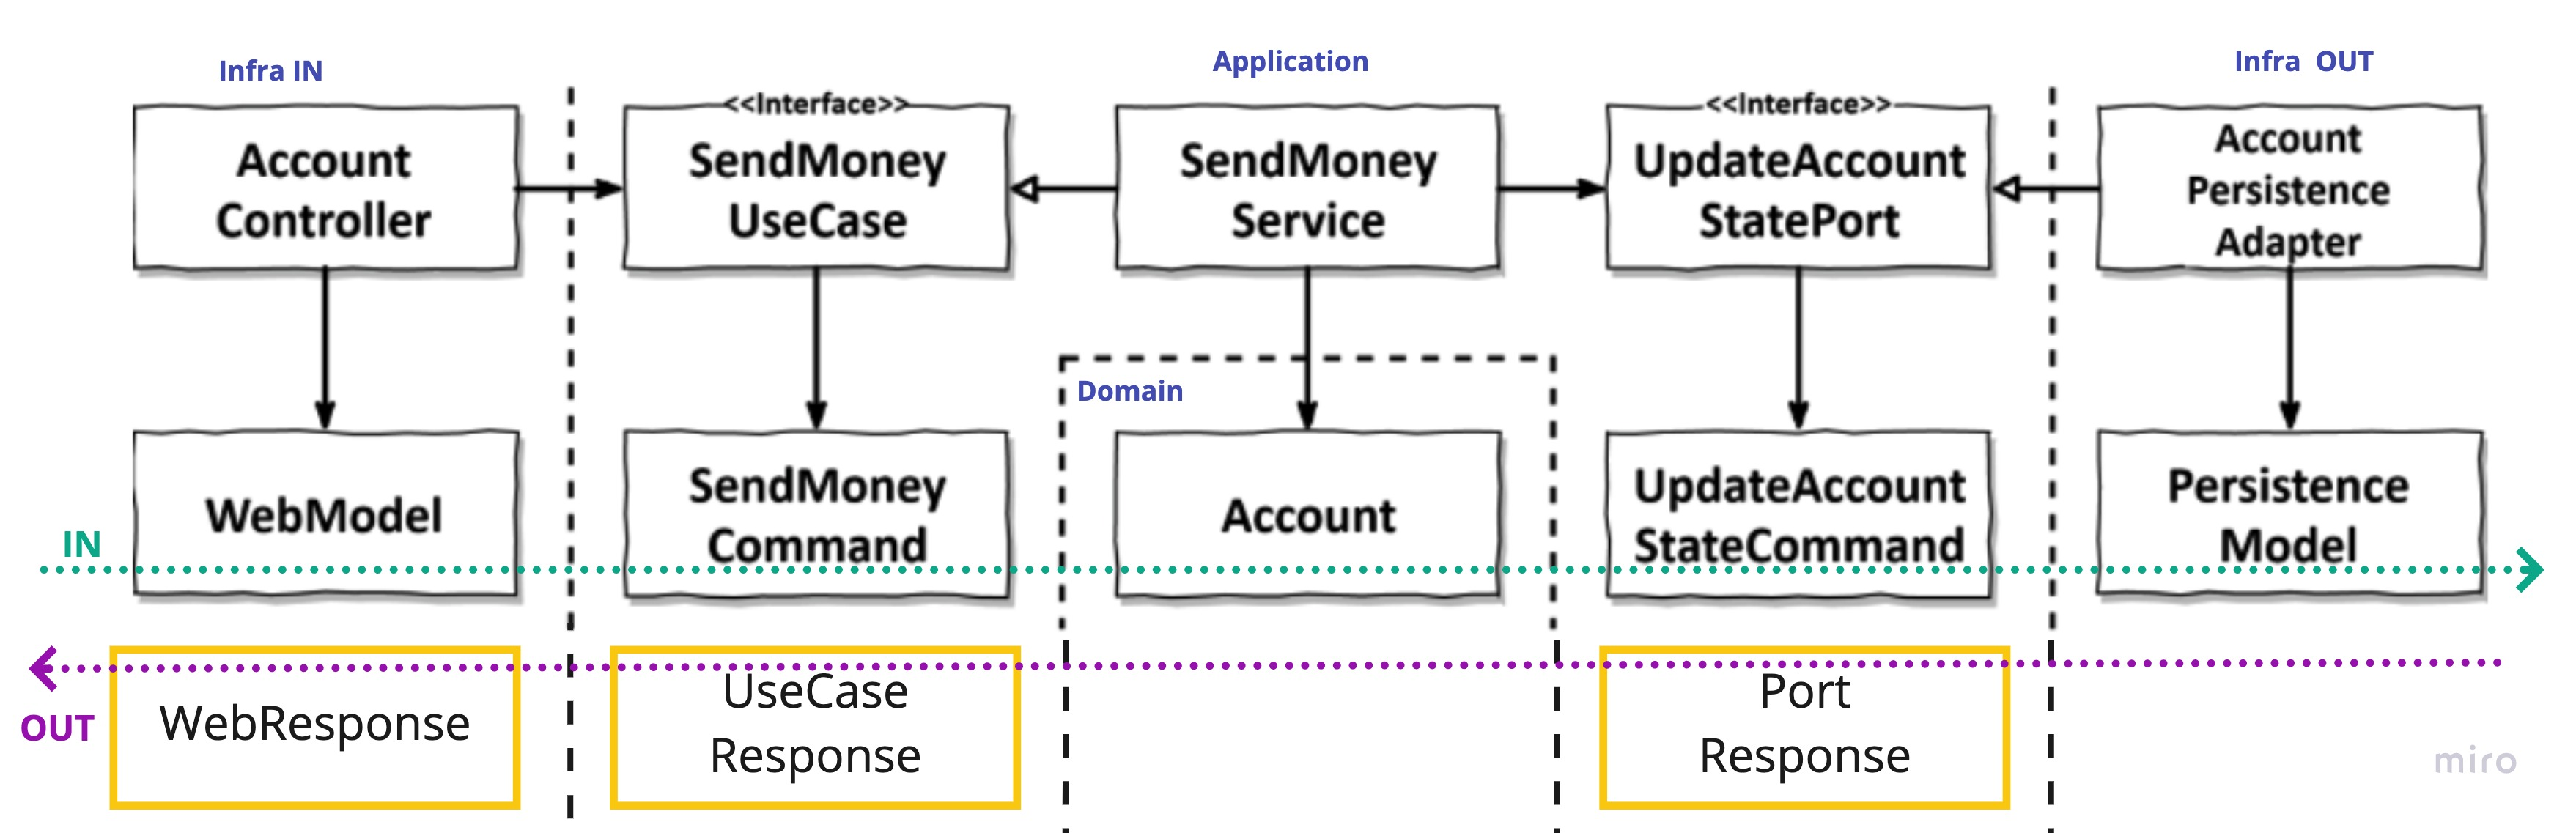
\includegraphics[height=0.2\textheight]{./part/Ejecucion/Seguimiento/CreateTaskUseCase/img/PFM - GetHandMapping}
    \caption{\textit{Full Mapping} con DTO de salida y de entrada\cite{TomHombergs2019GYHD}}\label{fig:GetHandMapping}
\end{figure}

\begin{figure}[H]
    \centering
    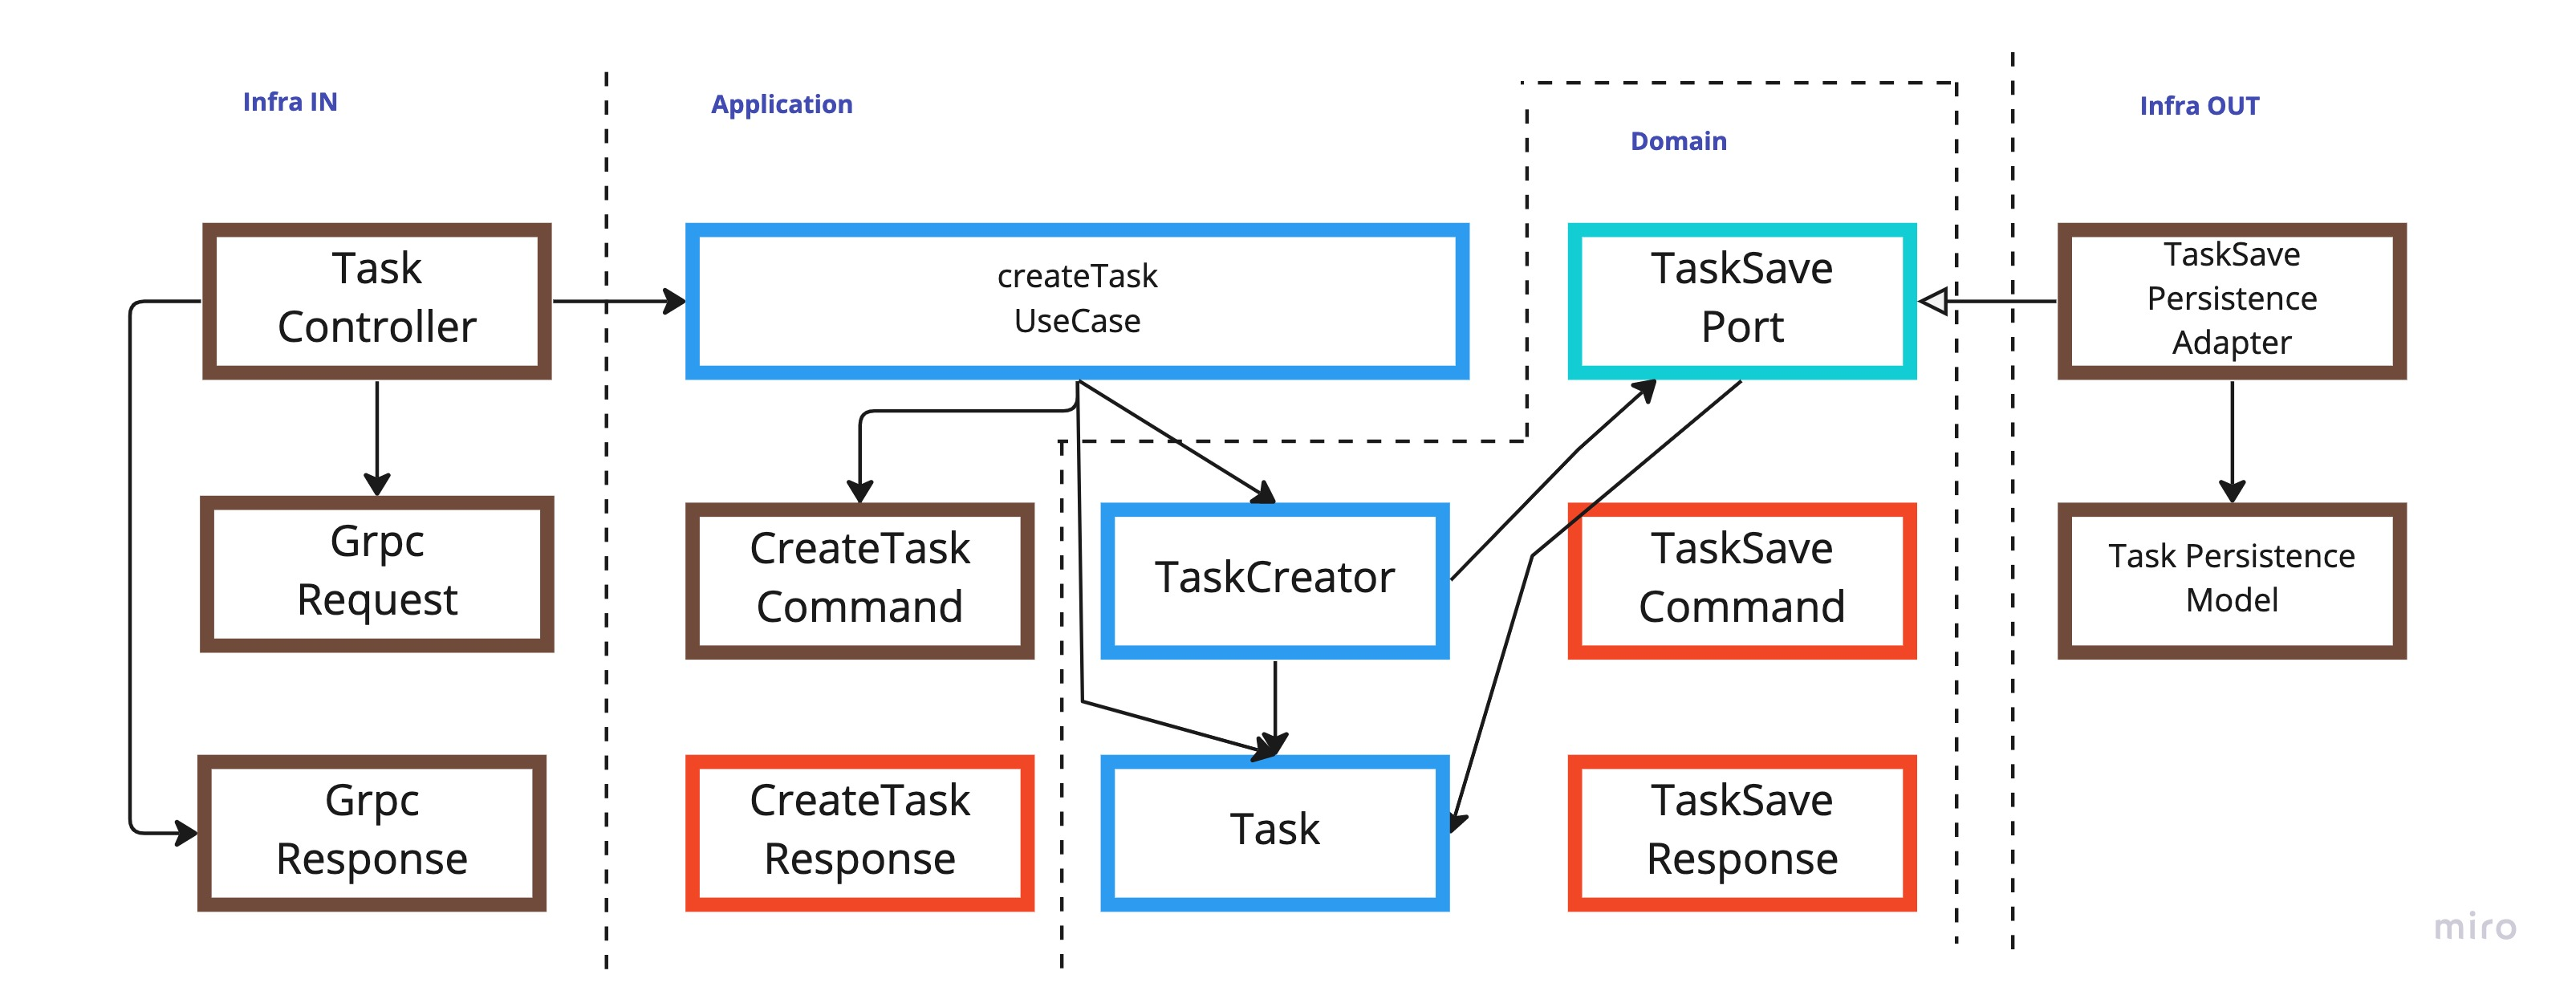
\includegraphics[height=0.2\textheight]{./part/Ejecucion/Seguimiento/CreateTaskUseCase/img/PFM - FinalMapping}
    \caption{\textit{CreateTaskUseCase Mapping} o Mapeo}\label{fig:CreateTaskUseCaseMapping}
\end{figure}

El código concreto para este caso de uso más relevante se compone de:
\begin{itemize}
    \item TaskController~\cref{lst:TaskControler}
    \item CreateTaskUseCase~\cref{lst:CreateTaskUseCaseCode}
    \item Creator~\cref{lst:Creator}
    \item SavePort~\cref{lst:SavePort}
    \item PersistAdapter~\cref{lst:SaveAdapter}
    \item DispatcherPort~\cref{lst:Dispatcher}
\end{itemize}

En el controller del~\cref{lst:TaskControler} se hace uso de la request entrante y se compone el comando que corresponde para el caso de uso.
Mediante la interfaz inyectada en el controller en el \textit{bootstrapping} se ejecuta el caso de uso resaltado en rojo.
También es interesante resaltar que una vez ejecutado el caso de uso se utiliza la respuesta, que contiene el id de la nueva Task creada para devolverlo.
Sin embargo, debido la estrategia utilizada de \textit{mapping}, definida en el diagrama~\cref{fig:CreateTaskUseCaseMapping}, no hacemos uso directo de esta respuesta si no que componemos una nueva para el protocolo de comunicación que está utilizando el cliente, en este caso RPC.
En los imports de este componente se aprecia que sólo hay dependencias de la infraestructura, gRPC en este caso, y de la capa de aplicación haciendo uso del comando y la interfaz del caso de uso.

La implementación del caso de uso se muestra en el~\cref{lst:CreateTaskUseCaseCode}.
Los imports son una forma rápida de comprobar la independencia de capas, de que la arquitectura, y de que los límites se están respetando.
En este caso todos corresponden a Dominio, no tiene imports de librerías de terceros, es decir, infraestructura.
La interfaz, utilizada en el controlador, \textit{UseCase} se encuentra escrita con la primera letra en mayúsculas, exponiéndola hacia afuera, mientras que el struct \textit{useCase} está en minúscula no pudiendo ser utilizado fuera del package.
El caso de uso realiza la instanciación de los \textit{ValueObjects} necesarios para la creación de una \textit{Task}.
Asegurando que no dan ningún error los datos de entrada y luego, haciendo uso del servicio se procede a crearla.
Aparece marcado en rojo el uso del servicio \textit{Creator} de Dominio.

En este caso se junta en un mismo fichero la interfaz y la implementación, al pertenecer a la misma capa.
No ocurre lo mismo dentro de \textit{Creator}~\cref{lst:Creator} Donde las interfaces de \textit{SaveRepository.Persist}~\cref{lst:SavePort} y \textit{Dispatcher.Dispatch}~\cref{lst:Dispatcher} se encuentra dentro del dominio, pero la implementación\textit{SaveAdapter}~\cref{lst:SaveAdapter} se encuentra en la capa de infraestructura.

El servicio de Dominio Creator se encarga de encapsular y atomizar los procesos que tienen que ocurrir en bloque siempre que se desee crear una Task.
Entre los cuales está: instanciar la tarea con los ValueObjects que recibe como parámetros;
Persistir la misma en la base de datos a través del puerto de salida, interfaz que implementará un adaptador;
y emitir el evento de creación a través del otro puerto de salida, el Dispatcher interfaz que implementará otro adaptador.
En la sección de \textit{imports} se aprecia que no hay elementos de infraestructura o aplicación.
Se limita al uso de Dominio.
Aislados del exterior.


\phantom{blank}
\vspace{5mm}
\hrule
\begin{lstlisting}[language=Go,caption={TaskController.go},breaklines=true,label={lst:TaskControler}]

package Controller

import (
	"context"
	"fmt"
	taskProto "github.com/Enrikerf/pfm/commandManager/app/Adapter/In/ApiGrcp/gen/task"
	"github.com/Enrikerf/pfm/commandManager/app/Application/Port/In/Task/CreateTask"
	"google.golang.org/grpc/codes"
	"google.golang.org/grpc/status"
)

type TaskController struct {
	SaveTaskUseCase   CreateTask.UseCase
}

func (controller TaskController) CreateTask(
	ctx context.Context,
	request *taskProto.CreateTaskRequest,
) (*taskProto.CreateTaskResponse, error) {
	protoTask := request.GetTaskParams()
	var command CreateTask.Command
	command.Host = protoTask.GetHost()
	command.Port = protoTask.GetPort()
	command.CommandSentences = protoTask.GetCommands()
	command.CommunicationMode = protoTask.GetMode().String()
	command.ExecutionMode = protoTask.GetExecutionMode().String()

    <@\textcolor{red}{task, err := controller.SaveTaskUseCase.Create(command)}@>

	if err != nil {
		return nil, fmt.Errorf("error")
	}
	var commandNames []string
	for _, command := range task.GetSteps() {
		commandNames = append(commandNames, command.GetSentence())
	}
	newTask := taskProto.Task{
		Uuid:          task.GetId().GetUuidString(),
		Host:          task.GetHost().GetValue(),
		Port:          task.GetPort().GetValue(),
		Commands:      commandNames,
		Mode:          string(task.GetCommunicationMode()),
		Status:        string(task.GetStatus().Value()),
		ExecutionMode: string(task.GetExecutionMode()),
	}
	return &taskProto.CreateTaskResponse{Task: &newTask}, nil
}

\end{lstlisting}
\hrule

\phantom{blank}
\vspace{5mm}
\hrule
\begin{lstlisting}[language=Go,caption={CreateTaskUseCase.go},breaklines=true,label={lst:CreateTaskUseCaseCode}]
package CreateTask

import (
	"github.com/Enrikerf/pfm/commandManager/app/Domain/Event"
	"github.com/Enrikerf/pfm/commandManager/app/Domain/Task"
	"github.com/Enrikerf/pfm/commandManager/app/Domain/Task/CommunicationMode"
	"github.com/Enrikerf/pfm/commandManager/app/Domain/Task/ExecutionMode"
	"github.com/Enrikerf/pfm/commandManager/app/Domain/Task/Host"
	"github.com/Enrikerf/pfm/commandManager/app/Domain/Task/Port"
	"github.com/Enrikerf/pfm/commandManager/app/Domain/Task/Repository"
	"github.com/Enrikerf/pfm/commandManager/app/Domain/Task/Service/Creator"
	"github.com/Enrikerf/pfm/commandManager/app/Domain/Task/Step"
)

type UseCase interface {
	Create(command Command) (Task.Task, error)
}

func New(saveRepository Repository.Save, dispatcher Event.Dispatcher) UseCase {
	return &useCase{Creator.Creator{
		SaveRepository: saveRepository,
		Dispatcher:     dispatcher,
	}}
}

type useCase struct {
	creator Creator.Creator
}

func (useCase *useCase) Create(command Command) (Task.Task, error) {
	host, err := Host.NewVo(command.Host)
	if err != nil {
		return nil, err
	}
	port, err := Port.NewVo(command.Port)
	if err != nil {
		return nil, err
	}
	communicationMode, err := CommunicationMode.FromString(command.CommunicationMode)
	if err != nil {
		return nil, err
	}
	executionMode, err := ExecutionMode.FromString(command.ExecutionMode)
	if err != nil {
		return nil, err
	}
	var stepVos []Step.Vo
	for _, commandSentence := range command.CommandSentences {
		stepVo, err := Step.NewVo(commandSentence)
		if err != nil {
			return nil, err
		}
		stepVos = append(stepVos, stepVo)
	}
	if err != nil {
		return nil, err
	}
	<@\textcolor{red}{return useCase.creator.Create(}@>
		<@\textcolor{red}{host,}@>
		<@\textcolor{red}{port,}@>
		<@\textcolor{red}{stepVos,}@>
		<@\textcolor{red}{communicationMode,}@>
		<@\textcolor{red}{executionMode,}@>
	<@\textcolor{red}{)}@>
}


\end{lstlisting}
\hrule

\phantom{blank}
\vspace{5mm}
\hrule
\begin{lstlisting}[language=Go,caption={Creator.go},breaklines=true,label={lst:Creator}]
package Creator

import (
	"github.com/Enrikerf/pfm/commandManager/app/Domain/Event"
	"github.com/Enrikerf/pfm/commandManager/app/Domain/Task"
	"github.com/Enrikerf/pfm/commandManager/app/Domain/Task/CommunicationMode"
	TaskEvent "github.com/Enrikerf/pfm/commandManager/app/Domain/Task/Event"
	"github.com/Enrikerf/pfm/commandManager/app/Domain/Task/ExecutionMode"
	"github.com/Enrikerf/pfm/commandManager/app/Domain/Task/Host"
	"github.com/Enrikerf/pfm/commandManager/app/Domain/Task/Port"
	"github.com/Enrikerf/pfm/commandManager/app/Domain/Task/Repository"
	"github.com/Enrikerf/pfm/commandManager/app/Domain/Task/Step"
)

type Creator struct {
	SaveRepository Repository.Save
	Dispatcher     Event.Dispatcher
}

func (creator *Creator) Create(
	host Host.Vo,
	port Port.Vo,
	stepVos []Step.Vo,
	communicationMode CommunicationMode.Mode,
	executionMode ExecutionMode.Mode,
) (Task.Task, error) {

	var task, err = Task.New(
		host,
		port,
		stepVos,
		communicationMode,
		executionMode,
	)
	if err != nil {
		return nil, err
	}
	creator.SaveRepository.Persist(task)
	creator.Dispatcher.Dispatch(TaskEvent.NewTaskCreated(task.GetId().GetUuidString()))

	return task, nil
}



\end{lstlisting}
\hrule

\phantom{blank}
\vspace{5mm}
\hrule
\begin{lstlisting}[language=Go,caption={SavePort.go},breaklines=true,label={lst:SavePort}]
package Repository

import "github.com/Enrikerf/pfm/commandManager/app/Domain/Task"

type Save interface {
	Persist(task Task.Task)
}


\end{lstlisting}
\hrule

\phantom{blank}
\vspace{5mm}
\hrule
\begin{lstlisting}[language=Go,caption={Dispatcher.go},breaklines=true,label={lst:Dispatcher}]
package Event

type Dispatcher interface {
	Dispatch(event Event)
}


\end{lstlisting}
\hrule

\phantom{blank}
\vspace{5mm}
\hrule
\begin{lstlisting}[language=Go,caption={SaveAdapter.go},breaklines=true,label={lst:SaveAdapter}]
package TaskAdapter

import (
	"github.com/Enrikerf/pfm/commandManager/app/Adapter/Out/Persistence/Model"
	"github.com/Enrikerf/pfm/commandManager/app/Domain/Task"
	"gorm.io/gorm"
)

type PersistAdapter struct {
	Orm *gorm.DB
}

func (adapter PersistAdapter) Persist(task Task.Task) {
	var currentTaskMysql Model.TaskDb
	var taskValuesToUpdate = Model.TaskDb{}
	taskValuesToUpdate.FromDomainV2(task)
	err := adapter.Orm.First(&currentTaskMysql, "uuid = ?", taskValuesToUpdate.Uuid).Error
	if err != nil {
		var taskMysql = Model.TaskDb{}
		taskMysql.FromDomainV2(task)
		_ = adapter.Orm.Create(&taskMysql).Error
	}
	adapter.Orm.Model(&currentTaskMysql).Updates(taskValuesToUpdate)
}


\end{lstlisting}
\hrule

